\documentclass[oneside, 12pt]{book}
\usepackage{icdthesisUTF}
\usepackage{tabularx} 
\usepackage{epsfig}
\usepackage[T1]{fontenc}
\usepackage[utf8]{inputenc}
\usepackage{array}
\usepackage{hyperref}
\usepackage[pdftex]{graphicx}
\usepackage{natbib} \DeclareGraphicsRule{*}{mps}{*}{}
\newcolumntype{P}[1]{>{\centering\arraybackslash}p{#1}}
\setcounter{tocdepth}{4}
\setcounter{secnumdepth}{4}
%Τα παρακάτω είναι υποχρεωτικά:

\renewcommand{\thesistitle}{Ανάπτυξη βιβλιοθήκης που επιτρέπει τον έλεγχο εφαρμογών μέσω φωνητικών εντολών}
\renewcommand{\thesisauthor}{Πετρόπουλος Ευάγγελος (3785)}
\renewcommand{\thesisauthorabbrv}{E. Πετρόπουλος}
\renewcommand{\thesisauthorinitials}{ΕΠ}
\renewcommand{\thesissupervisor}{Ν. Πεταλίδης}
\renewcommand{\thesismonth}{Μάϊος}
\renewcommand{\thesisyear}{2020}

% Μόνο αν η συγγραφέας είναι γυναίκα 
%\renewcommand{\thesisauthorsex}{female} %if author is female

%Μόνο αν οι συγγραφείς είναι δύο:
%\renewcommand{\thesisSecondAuthor}{Κάποιου άλλου (200)}
%\renewcommand{\thesisSecondAuthorabbrv}{K. άλλος}
%\renewcommand{\thesisSecondAuthorInitials}{ΚΑ}
% Η βιβλιογραφία
\addbibresource{testUTF.bib}

\begin{document}
% Υποχρεωτικά τα παρακάτω:
\Titlepage
\Declarationpage
\begin{Abstract}
  Οι μελισσοκόμοι καταγράφουν σημειώσεις για τα μελίσσια που ελέγχουν αλλά πολλές φορές δεν
  προλαβαίνουν επειδή ο αριθμός των μελισσιών είναι μεγάλος ή δουλέυουν μόνοι τους και πρέπει να
  σταματάνε την εργασία για να καταγράψουν τις σημειώσεις.Η εφαρμογή που αναπτύξαμε και ονομάζεται
  ConApi (Contemporary Apiculture) υλοποιεί ένα σύστημα φωνητικών εντολών που βοηθάνε τον
  μελισσοκόμο στην καταγραφή των σημειώσεων χωρίς την χρήση της συσκευής με τα χέρια παρά μονο της
  φωνής.
\end{Abstract}
\tableofcontents

%Μόνο εφόσον θέλετε χωριστό πίνακα για εικόνες και πίνακες
\listoftables
\listoffigures

%Προαιρετικά
\begin{Preface}
Εδώ μπορεί να μπει πρόλογος. (Δεν είναι απαραίτητο).
\end{Preface}

%Προαιρετικά
\begin{Acknowledgement}
Ευχαριστίες (στο μπαμπά, στη μαμά, κτλ)
\end{Acknowledgement}

%Προαιρετικά
\begin{Definitions}
Ορισμοί εννοιών που μπορεί να είναι χρήσιμοι. Για παράδειγμα:

\begin{description}
\item [\LaTeX] Σύστημα στοιχειοθεσίας κειμένων
\end{description}

\end{Definitions}

%Από εδώ αρχίζει το κείμενό σας
\chapter{Εισαγωγή}\label{ch:εισαγωγή}
\leftmark\rightmark
Η μελισσοκομία είναι μια επιστήμη που οι άνθρωποι ασχολούνται από τα αρχαία χρόνια και μία απο τις
δουλειές είναι ο τακτικός έλεγχος για την πρόοδο των μελισσιών.
Σε κάθε έλεγχο του μελισσιού καταγράφουν χειρόγραφες σημειώσεις για την πρόοδο του.
Οι σημειώσεις είτε γράφονται παράλληλα με τον έλεγχο των μελλισιών είτε μέτα το πέρας του έλεγχου. \par
Δυσκολίες συναντιούνται με την καταγραφή των χειρόγραφων σημειώσεων, όπως στο μεγάλο αριθμό μελισσιών
ο μελισσοκόμος να μην προλαβαίνει να καταγράφει τις παρατηρήσεις του απο τον έλεγχο, να ξεχνάει τι
είχε παρατηρήσει στα μελίσσια στην αρχή του ελέγχου.
Επιπλέον ο μελισσοκόμος φοράει ειδική στολή (μάσκα, γάντια) που καθιστούν δύσκολη την καταγραφή των
παρατηρήσεων όπως με την μάσκα δεν θα βλέπει καλά λόγο της σίτας που έχει, επίσης με τα γάντια
υπάρχει δυσκόλια στον να κρατήσει το μολύβι, το τετράδιο και να καταγράψει τις σημειώσεις. \par
Για τους παραπάνω λόγους είναι ενδιαφέρουσα η ανάπτυξη ενός εργαλείου το οποίο θα λύνει τα χέρια του
μελισσοκόμου χρησιμοποιώντας μόνο την φωνή του για την καταγραφή των παρατηρήσεων. \par
Σκοπός αυτής της εργασίας είναι η ανάπτυξη ένος τέτοιου εργαλείου που θα υποστηρίζει φωνητικές
εντολές για την ευκολία καταγραφής των παρατηρήσεων.

\section{Δομή της εργασίας}\label{sec:δομή-της-εργασίας}
\noindent
\textbf{Κεφάλαιο 2}\quad Παρουσίαση έλεγχου μελισσιών και χειρόγραφες σημειώσεις.\newline
\textbf{Κεφάλαιο 3}\quad Εφαρμογή και φωνητικές εντολές.\newline
\textbf{Κεφάλαιο 4}\quad Speech-to-Text API.

\chapter{Έλεγχος μελισσιών και χειρόγραφες σημειώσεις}
\label{ch:έλεγχος-μελισσιών-και-χειρόγραφες-σημειώσεις}
\section{Έλεγχος}
\label{sec:έλεγχος}
Ο έλεγχος των μελισσιών πραγματοποιείται όλες τις εποχές του χρόνου.
Ο μελισσοκόμος μετά απο τον Χειμώνα, στην αρχή της Άνοιξης θα κάνει τον πρώτο έλεγχο των μελισσιών
που θα κοιτάξει αν η βασίλισσα του μελισσιού είναι ζωντανή και αν γεννάει γόνο.
Στα μέσα της Άνοιξης θα ελέγξει αν ο γόνος αυξήθηκε, αν έιναι συμπαγής και πόσα πλαίσια γόνου έχει το
μελίσσι.\par
Την επόμενη εποχή, το καλοκαίρι με τους ελέγχους που θα κάνει θα παρατηρήσει αν τα μελίσσια συλλέγουν
μέλι και αν η βασίλισσα σταμάτησε να γεννάει γόνο.
Προς το τέλος του καλοκαιριού θέλει να δεί αν έχουν συλλέξει αρκετό μέλι για να γίνει ο τρύγος.\par
Το Φθινόπωρο γίνεται έλεγχος για να διακρίνει αν η βασίλισσα γεννάει συμπαγή γόνο και το Χειμώνα αν
τα μελίσσια έχουν ασθένειες.
\section{Χειρόγραφες σημειώσεις}
\label{sec:χειρόγραφες-σημειώσεις}
Οι χειρόγραφες σημειώσεις του μελισσοκόμου αποτελούνται από τον αριθμό της κυψέλης και την ηλικία της
βασίλισσας.
Επιπλέον, σε κάθε έλεγχο καταγράφεται η ημερομηνία, πόσα πλαίσια έχει η κυψέλη και από τα
οποία πόσα έχουν πληθυσμό.
Επίσης, καταγράφεται απο τα πλαίσια πόσα έχουν γόνο, μέλι και γύρη.
Τέλος, σημειώνονται γενικές παρατηρήσεις/υπενθυμίσεις της κυψέλης.

\begin{table}[h]
  \centering
  \caption{Ημερολόγιο Μελισσοκόμου.}
  \begin{tabularx}{\linewidth}[h]{|P{2cm}|P{1.5cm}|P{2cm}|P{1cm}|P{1cm}|P{1cm}|P{3cm}|}
    \hline
    \multicolumn{3}{|l|}{Αριθμός Κυψέλης: 6} & \multicolumn{4}{l|}{Ηλικία Βασίλισσας: 05-2019} \\
    \hline
    Ημερομηνία&Πλαίσια&Πληθυσμός&Γόνος&Μέλι&Γύρη&Παρατηρήσεις\\
    \hline
    09-04-2019&10&7&4&&&OK\\
    \hline
    18-04-2019&10&10&7&&&Θέλει όροφο\\
    \hline
    24-04-2019&15&10&8&&&2 πλαίσια έχουν βασιλικά κελιά, μπήκε όροφος\\
    \hline
    03-05-2019&15&10&8&&&Έκοψα παραφιάδα Ν10\\
    \hline
  \end{tabularx}
  \label{tab:table2}
\end{table}
\section{Δυσκολίες}\label{sec:δυσκολίες}
Οι μελισσοκόμοι συναντάνε δυσκολίες στο να κρατάνε τις σημειώσεις τους.
Μια απο αυτές τις δυσκολίες είναι η στολή που χρησιμοποιούν, η οποία αποτελείται απο την μάσκα, την
φόρμα και τα γάντια.
Η μάσκα έχει τούλι στο να επιτρέπει τον μελισσοκόμο να βλέπει και να εμποδίζει τις μέλισσες να
εισέλθουν μέσα στην μάσκα.
Το τούλι της μάσκας δυσκολεύει την διαδικάσια καταγραφείς των σημειώσεων διότι εμποδίζει στο να
βλέπεις καθαρά το τετραδιο.
Τα μελισσοκομικά γάντια αποτρέπουν τις μέλισσες από τσιμπήματα στα χέρια αλλά δυσκολεύουν στο
κράτημα του μολυβιού ώστε να γράφτούν οι σημειώσεις στο τετράδιο.
\chapter{Εφαρμογή και φωνητικές εντολές}
\label{ch:εφαρμογή-και-φωνητικές-εντολές}
\section{Εφαρμογή}
\label{sec:εφαρμογή}
Η εφαρμογή που υλοποιείται σε αυτή την εργασία δύναται να λύσει τις δυσκολίες που αντιμετωπίζει ο
μελισσοκόμος.
Όπως αναφέραμε παραπάνω η δυσκολία που συναντάει ο μελισσοκόμος είναι η καταγραφή των σημειώσεων που
είναι σημαντικές για την πρόοδο των μελισσιών.
Η εφαρμογή κρατάει τα δεδομένα όπως παρουσιάζονται στο παραπάνω πίνακα~\ref{tab:table2}.
Συγκεκριμένα, οι εγγραφές για όλα τα μελίσσια που δουλεύει ο μελισσοκόμος. \newline
Για κάθε μελίσσι τα δεδομένα είναι:
\begin{itemize}
  \item Αριθμός Κυψέλης
  \item Ηλικία Βασίλισσας
  \item Ημερομηνία (κάθε ελέγχου)
  \item Πλαίσια (αριθμός πλαίσιων κυψέλης)
  \item Πληθυσμός κυψέλης (αριθμός πλαίσιων με μέλισσες)
  \item Γόνος (αριθμός πλαίσιων με γόνο)
  \item Μέλι (αριθμός πλαίσιων με μέλι)
  \item Γύρη (αριθμός πλαίσιων με γύρη)
  \item Παρατηρήσεις
\end{itemize}
Η εφαρμογή με την υλοποιήση ενός γραφικού περιβάλλοντος για την προβολή και επεξεργασία των
μελισσοκομικών δεδομένων και την υλοποιήση μιας διεπαφής χρήστη φωνής με φωνητικές εντολές για την
καταχώρηση των μελισσοκομικών δεδομένων λύνοντας τις δυσκολίες που αντιμετωπίζει ο μελισσοκόμος κατά
τη διάρκεια της εργασίας.
\section{GUI-Γραφικό περιβάλλον διεπαφής χρήστη}
\label{sec:gui-γραφικό-περιβάλλον-χρήστη}
Το γραφικό περιβάλλον της εφαρμογής θα παρουσίαζει με ωραία γραφικά τα μελίσσια και κάθε πληροφορία
του μελισσιού και θα δίνει δυνατότητα στον χρήστη να επεξεργαστεί αυτή την πληροφορία.
\section{VUI-Διεπαφή χρήστη φωνής}
\label{sec:vui---διεπαφή-χρήστη-φωνής}
\section{Φωνητικές Εντολές}
\label{sec:φωνητικές-εντολές}
Δυο κατηγορίες φωνητικών εντολών υποστηρίζονται, οι οποίες είναι:
\begin{enumerate}
  \item Μελισσιού
  \item Έλεγχος μελισσιού
\end{enumerate}
Οι φωνητικές εντολές κατά τον έλεγχο του μελισσιού θα ενεργοποιούνται όταν επιλεχθεί το μελίσσι για έλεγχο.
Οι φωνητικές εντολές της εφαρμογής είναι:
\begin{table}[h]
  \centering
  \caption{Φωνητικές εντολές}
  \begin{tabularx}{\linewidth}[h]{|X|X|X|}
    \hline
    Φωνητικές Εντολές & Περιγραφή & Παράδειγμα \\
    \hline
    \hline
    Μελίσσι <αριθμός> & Στο πεδίο <αριθμός> θα λέγεται ο αριθμός του μελισσιού & Μελίσσι 6 \\
    \hline
    Πλαίσια <αριθμός> & Στο πεδίο <αριθμός> θα λέγεται ο αριθμός των πλαίσιων του μελισσιού & Πλαίσια 10 \\
    \hline
    Πληθυσμός <αριθμός> & Στο πεδίο <αριθμός> θα λέγεται ο αριθμός των πλαίσιων με πληθυσμό του μελισσιού & Πληθυσμός 7 \\
    \hline
    Γόνος <αριθμός> & Στο πεδίο <αριθμός> θα λέγεται ο αριθμός των πλαίσιων με γόνο του μελισσιού & Γόνος 4 \\
    \hline
    Μέλι <αριθμός> & Στο πεδίο <αριθμός> θα λέγεται ο αριθμός των πλαίσιων με μέλι του μελισσιού & Μέλι 3 \\
    \hline
    Γύρη <αριθμός> & Στο πεδίο <αριθμός> θα λέγεται ο αριθμός των πλαίσιων με γύρη του μελισσιού & Γύρη 3 \\
    \hline
    Παρατηρήση <κείμενο> & Στο πεδίο <κείμενο> θα λέγεται η παρατήρηση για το μελίσσι & Παρατήρηση Θέλει όροφο  \\
    \hline
  \end{tabularx}
  \label{tab:table3}
\end{table}
\chapter{Ανασκόπηση Speech-to-Text APIs}
\label{ch:ανασκόπηση-speech-to-text-apis}
\section{APIs}
\label{sec:apis}
\subsection{Google Could Speech-to-Text API}
\label{subsec:google-speech-to-text}
\subsubsection{Περιγραφή}
Είναι ένα API μεταγραφής ομιλίας σε κείμενο υποστηριζοντάς πολλές γλώσσες προγραμματισμού, γεγονός
που το καθιστά ανεξάρτητο πλατφόρμας.
Το API που υποστηρίζεται από τις τεχνολογίες AI της Google και έχει την δυνατότητα χρήσης
διαφορετικών μοντέλων μηχανικής εκμάθησης για αιτήματα μεταγραφής ήχου σε Speech-to-Text.
\subsubsection{Δυνατότητες}
\begin{itemize}
  \item \textbf{Παγκόσμιο λεξιλόγιο} - Εκτεταμένη υποστήριξη γλώσσας ομιλίας σε κείμενο σε περισσότερες από 125 γλώσσες και παραλλαγές.
  \item \textbf{Ροή αναγνώριση ομιλίας} - Αποτελέσματα αναγνώρισης ομιλίας σε πραγματικό χρόνο καθώς το API επεξεργάζεται την είσοδο ήχου που μεταδίδεται σε ροή από το μικρόφωνο της εφαρμογής σας ή αποστέλλεται από ένα προκαθορισμένο αρχείο ήχου (inline ή μέσω Cloud Storage).
  \item \textbf{Προσαρμογή ομιλίας} - Προσαρμογή της αναγνώρισης ομιλίας για την μετατροπή ορών για συγκεκριμένους τομείς και σπάνιες λέξεις παρέχοντας συμβουλές και ενισχύση της ακρίβεις της μεταγραφής συγκεκριμένων λέξεων ή φράσεων. Αυτόματη μετατροπή προφορικών αριθμών σε διευθύνσεις, έτη, νομίσματα και άλλα χρησιμοποιώντας τάξεις.
  \item \textbf{Πολυκαναλική αναγνώριση} - Το Speech-to-Text μπορεί να αναγνωρίσει διαφορετικά κανάλια σε καταστάσεις πολλαπλών καναλιών (π.χ., τηλεδιάσκεψη) και να σχολιάσει τις μεταγραφές για τη διατήρηση της τάξης.
  \item \textbf{Ανθεκτικότητα θορύβου} - Το Speech-to-Text μπορεί να χειριστεί θορυβώδη ήχο από πολλά περιβάλλοντα χωρίς να απαιτείται επιπλέον ακύρωση θορύβου.
  \item \textbf{Μοντέλα ειδικά για τομέα} - Επιλέξτε από μια επιλογή εκπαιδευμένων μοντέλων για φωνητικό έλεγχο και τηλεφωνική κλήση και μεταγραφή βίντεο βελτιστοποιημένη για απαιτήσεις ποιότητας για συγκεκριμένο τομέα. Για παράδειγμα, το βελτιωμένο μοντέλο τηλεφωνικών κλήσεων είναι συντονισμένο για ήχο που προέρχεται από την τηλεφωνία, όπως οι τηλεφωνικές κλήσεις που έχουν εγγραφεί σε ρυθμό δειγματοληψίας 8khz.
  \item Υποστηρίζει γλώσσες προγραμματισμού όπως Protocol, C#, Go, java, Node.js, PHP, Python και Ruby.
\end{itemize}

Λαμβάνοντας υπόψη ότι η Google είναι ουσιαστικά το νευρικό σύστημα του Διαδικτύου σε αυτό το σημείο, δεν αποτελεί έκπληξη ότι το API ομιλίας σε κείμενο είναι ένα από τα πιο δημοφιλή - και πιο ισχυρά - API που είναι διαθέσιμα στους προγραμματιστές.

Το Google Speech-To-Text παρουσιάστηκε το 2018, μόλις μία εβδομάδα μετά την ενημέρωση κειμένου σε ομιλία. Το API Speech-To-Text της Google προβάλλει ορισμένες τολμηρές αξιώσεις, μειώνοντας τα λάθη λέξεων κατά 54\% σε δοκιμή μετά τη δοκιμή. Σε ορισμένους τομείς, τα αποτελέσματα είναι ακόμη πιο ενθαρρυντικά.

Ένας από τους λόγους για την εντυπωσιακή ακρίβεια των API είναι η δυνατότητα επιλογής μεταξύ διαφορετικών μοντέλων μηχανικής εκμάθησης, ανάλογα με το τι χρησιμοποιείται η εφαρμογή σας. Αυτό καθιστά επίσης το Google Speech-To-Text μια κατάλληλη λύση για εφαρμογές εκτός από τις σύντομες αναζητήσεις ιστού. Μπορεί επίσης να ρυθμιστεί για ήχο από τηλεφωνικές κλήσεις ή βίντεο. Υπάρχει επίσης μια τέταρτη ρύθμιση, την οποία συνιστά η Google να χρησιμοποιείται ως προεπιλογή.

Το API ομιλίας σε κείμενο διαθέτει επίσης μια εντυπωσιακή ενημέρωση για επιλογές εκτεταμένων σημείων στίξης. Αυτό έχει σχεδιαστεί για να κάνει πιο χρήσιμες μεταγραφές, με λιγότερες τρέχουσες προτάσεις ή σφάλματα στίξης.

Η πιο πρόσφατη ενημέρωση επιτρέπει επίσης στους προγραμματιστές να προσθέσουν ετικέτες στον ήχο ή το βίντεο που έχουν μεταγραφεί με βασικά μεταδεδομένα. Αυτό είναι περισσότερο προς όφελος της εταιρείας παρά για τους προγραμματιστές, ωστόσο, καθώς θα επιτρέψει στην Google να αποφασίσει ποιες λειτουργίες είναι πιο χρήσιμες για τους προγραμματιστές.

Το Google Speech-To-Text API δεν είναι, ωστόσο, δωρεάν. Είναι δωρεάν για αναγνώριση ομιλίας για ήχο λιγότερο από 60 λεπτά. Για μεταγραφές ήχου περισσότερο από αυτό, κοστίζει 0,006  ανά 15 δευτερόλεπτα.

\textbf{Πλεονεκτήματα}
\begin{itemize}
  \item Αναγνωρίζει πάνω από 120 γλώσσες
  \item Πολλαπλά μοντέλα μηχανικής εκμάθησης για αυξημένη ακρίβεια
  \item Αυτόματη αναγνώριση γλώσσας
  \item Μεταγραφή κειμένου
  \item Σωστή αναγνώριση ουσιαστικών
  \item Ιδιωτικότητα δεδομένων
  \item Ακύρωση θορύβου για ήχο από τηλεφωνικές κλήσεις και βίντεο
\end{itemize}
\textbf{Μειονεκτήματα}
\begin{itemize}
  \item Κοστίζει χρήματα
  \item Περιορισμένο πρόγραμμα δημιουργίας λεξιλογίου
\end{itemize}
\subsection{Microsoft Cognitive Services Speech-to-Text API}
\label{subsec:microsoft-cognitive-services-speech-to-text-api}
\subsubsection{Περιγραφή}
Microsoft Cognitive Services παρέχουν την μεταγραφή ομιλίας σε κείμενο από την υπηρεσία ομιλίας,
γνωστή και ως αναγνώριση ομιλίας, επιτρέπει τη μεταγραφή ροών ήχου σε κείμενο σε πραγματικό χρόνο.
Είναι επίσης ένα μέρος των υπηρεσιών Microsoft Trust που προσφέρουν ασύγκριτες επιλογές ασφάλειας
για προγραμματιστές που αναζητούν τα πιο ασφαλή δεδομένα για τις εφαρμογές τους.
Το κύριο πράγμα που διαχωρίζει το Microsoft Cognitive Services ’Speech to Text API είναι η
λειτουργία Αναγνώρισης Ομιλιτή.
Μπορεί να πραγματοποιήσει μεταγραφή σε πραγματικό χρόνο.
\subsubsection{Δυνατότητες}
\noindent
\textbf{Πλεονεκτήματα}
\begin{itemize}
  \item Βελτιωμένη ασφάλεια δεδομένων μέσω αλγορίθμων αναγνώρισης φωνής
  \item Μεταγραφή σε πραγματικό χρόνο
  \item Μετάφραση σε πραγματικό χρόνο
  \item Προσαρμόσιμο λεξιλόγιο
  \item Δυνατότητες κειμένου σε ομιλία για φυσικά πρότυπα ομιλίας
\end{itemize}
\textbf{Μειονεκτήματα}
\begin{itemize}
  \item Ενσωματωμένοι περιορισμοί λόγω της δημιουργίας του API για γενικούς σκοπούς
  \item Χρησιμοποιεί μικροσυσκευές, οι οποίες μπορεί να είναι χρήσιμες για την επίλυση μεμονωμένων προβλημάτων, αλλά δεν ανταποκρίνονται σε μεγαλύτερα προβλήματα
\end{itemize}
\subsection{IBM Watson API}
\label{subsec:ibm-watson}
\subsubsection{Πειργραφή}
Το Watson Speech to Text είναι μια λύση εγγενής στο cloud που χρησιμοποιεί αλγόριθμους AI βαθιάς
μάθησης για την εφαρμογή γνώσεων σχετικά με τη γραμματική, τη δομή της γλώσσας και τη σύνθεση ήχου /
φωνητικού σήματος για τη δημιουργία προσαρμόσιμης αναγνώρισης ομιλίας για βέλτιστη μεταγραφή
κειμένου.
\subsubsection{Δυνατότητες}
\textbf{Πλεονεκτήματα}
\begin{itemize}
  \item Επεξεργάζεται μη δομημένα δεδομένα
  \item Βοηθά τους ανθρώπους αντί να τους αντικαθιστούν
  \item Βοηθά να ξεπεραστούν οι ανθρώπινοι περιορισμοί
  \item Βελτιώνει την παραγωγικότητα παρέχοντας σχετικά δεδομένα
  \item Βελτιώνει την εμπειρία χρήστη
  \item Μπορεί να επεξεργαστεί μεγάλες ποσότητες δεδομένων
  \item Εύκολη εγκατάσταση και έναρξη
\end{itemize}
\textbf{Μειονεκτήματα}
\begin{itemize}
  \item Δεν υποστηρίζει άμεσα δομημένα δεδομένα
  \item Ακριβές για μετάβαση σε
  \item Απαιτείται συντήρηση
  \item Υποστηρίζει μόνο περιορισμένο αριθμό γλωσσών
  \item Χρειάζεται χρόνος για πλήρη εφαρμογή
  \item Απαιτεί εκπαίδευση και κατάρτιση για να αξιοποιήσει πλήρως τους πόρους της
\end{itemize}
\section{Επιλογή API}
\label{sec:επιλογή-api}
Στην προηγούμενη ενότητα περιγράψαμε τρία APIs. Το κάθε ένα είναι ικανό για μετραγραφή ομιλίας σε
κείμενο.
Όλα τα APIs εφαρμόζουν Machine learning και AI τεχνολογίες.
Το καθένα API έχει τα διαχωριστικά σημεία.

Το κύριο πράγμα που διαχωρίζει το Microsoft Cognitive Services ’Speech to Text API είναι η
λειτουργία Αναγνώρισης Ομιλητή.
Αυτή είναι η ακουστική έκδοση του λογισμικού ασφαλείας, όπως η αναγνώριση προσώπου.
Σκεφτείτε το ως σάρωση αμφιβληστροειδούς για τον ήχο της φωνής του χρήστη.
Το καθιστά απίστευτα εύκολο για διαφορετικά επίπεδα χρηστών.
Αυτή η ίδια δυνατότητα αναγνώρισης φωνής επιτρέπει στο λογισμικό να προσαρμόζεται στα συγκεκριμένα
στυλ και μοτίβα ομιλίας του χρήστη.
Προσφέρει επίσης περισσότερες προσαρμοσμένες επιλογές λεξιλογίου από το Google, ως επιπλέον
πλεονέκτημα.

Το IBM Watson Speech to Text API είναι ιδιαίτερα ανθεκτικό στην κατανόηση τα συμφραζόμενα,
στηρίζεται στη δημιουργία υποθέσεων και στην αξιολόγηση στη διαμόρφωση της απόκρισης.
Είναι επίσης σε θέση να κάνει διάκριση μεταξύ πολλαπλών ομιλητών, γεγονός που το καθιστά κατάλληλο
για τις περισσότερες εργασίες μεταγραφής.
Μπορείτε ακόμη και να ορίσετε έναν αριθμό φίλτρων, εξαλείφοντας βωμολοχίες, προσθέτοντας εμπιστοσύνη
λέξεων και επιλογές μορφοποίησης για εφαρμογές ομιλίας σε κείμενο.

Ένας από τους λόγους για την εντυπωσιακή ακρίβεια των API είναι η δυνατότητα επιλογής μεταξύ
διαφορετικών μοντέλων μηχανικής μάθησης, ανάλογα με το τι χρησιμοποιείται η εφαρμογή σας.
Αυτό καθιστά επίσης το Google Speech-To-Text μια κατάλληλη λύση για εφαρμογές εκτός από τις σύντομες
αναζητήσεις ιστού.
Μπορεί επίσης να ρυθμιστεί για ήχο από τηλεφωνικές κλήσεις ή βίντεο.
Υπάρχει επίσης μια τέταρτη ρύθμιση, την οποία συνιστά η Google να χρησιμοποιείται ως προεπιλογή.
Το API Speech-To-Text διαθέτει επίσης μια εντυπωσιακή ενημέρωση για εκτεταμένες επιλογές στίξης.
Αυτό έχει σχεδιαστεί για να κάνει πιο χρήσιμες μεταγραφές, με λιγότερες τρέχουσες προτάσεις ή
σφάλματα στίξης.
Επίσης το Google cloud Speech-to-Text API αναγνωρίζει πάνω από 120 γλώσσες συμπεριλαμβάνοντας και
την Ελληνική γλώσσα που χρησιμοποιείτε για την ανάπτυξη της βιβλιοθήκης.

\chapter{Σχεδίαση Βιβλιοθήκης}
\label{ch:σχεδίαση-βιβλιοθήκης}
\newpage
\includegraphics[scale=0.5]{figures/library_uml_diagram.eps}
%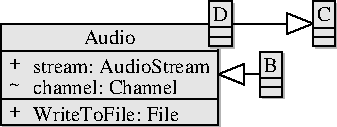
\includegraphics[scale=1]{figures/api_diagram-1.pdf} \\ \vspace{20cm} \\


%\section{Η τυπογραφία σήμερα}\label{sec:η-τυπογραφία-σήμερα}
%%Αυτή είναι η αναφορά σε ένα άρθρο περιοδικού:\citep{Schmidt98}.Αυτή
%%είναι η αναφορά σε ένα βιβλίο:\citep{goosens93}. Αυτή είναι η αναφορά
%%σε ένα ελληνικό βιβλίο:\citep{Chatzigeorgiou05}. Βιβλίο στα ελληνικά
%%με ξένο συγγραφέα:\citep{Sommerville09}. Άρθρο σε
%%συνέδριο~\citep{4343930}.
%
%Τέλος αναφορά σε ιστοσελίδα:~\citep{Wikipedia_BibTeX}.

%Εδώ αναφερόμαστε στo σχήμα~\ref{fig:image1}:
%\begin{figure}[h]
%  \centering
%  
\includegraphics[width=35mm]{lion.png}
%  \caption{Παράδειγμα εικόνας}
%  \label{fig:image1}
%\end{figure}
%dsasdadadasdasdas
%ad
%asd
%asd
%
%και εδώ στον πίνακα~\ref{tab:table1}:
%\begin{table}[h]
%  \centering
%  \caption{Παράδειγμα πίνακα}
% \begin{tabularx}{\linewidth}[h]{|XXX|}%
%\hline
%\hline
%Κίνητρα & Παραδείγματα ευρημάτων & Αριθμός μελετών\\
%\hline
%Ταύτιση με το έργο & Ξεκάθαροι στόχοι &20\\
%Καλό management & Ομαδικότητα &16\\
%Συμμετοχή υπαλλήλων & Συμμετοχή στις αποφάσεις&16\\
%Προοπτικές εξέλιξης & Προοπτικές προαγωγής&15\\
%Ποικιλία στην εργασία & Καλή χρήση ικανοτήτων& 14\\
%Αίσθηση του να ανήκεις κάπου& Υποστηρικτικές σχέσεις&14\\
%Αμοιβές και κίνητρα & Αυξημένος μισθός& 14\\
%\hline
%\hline
%\end{tabularx}
%  \label{tab:table1}
%\end{table}
%\appendix
%\chapter{Συνοπτικός οδηγός χρήσης \LaTeX}
%Εδώ βάζετε ότι θα έμπαινε σε παράρτημα.
%\texttt{Δοκιμή σε mono-space}
%Προαιρετικά
\begin{Glossary}
Το γλωσσάρι μπορεί να είναι χρήσιμο αν χρησιμοποιείτε πολλά ακρώνυμα
και συντομογραφίες. Για παράδειγμα

https://nordicapis.com/5-best-speech-to-text-apis/
\newline
https://cloud.google.com/speech-to-text\#all-features
\newline
https://www.ibm.com/cloud/watson-speech-to-text
\newline
https://azure.microsoft.com/en-us/services/cognitive-services/speech-to-text/
\begin{description}
\item[TCP]Transmission Control Protocol
\end{description}
\end{Glossary}

\printbibliography
\lastpageinfo
\end{document}
